\leftsection{Программа 2}

\subsection{Однопоточная программа}

\begin{lstlisting}[language=c, caption={Вторая программа (однопоточный вариант)}]
#include <stdlib.h>
#include <stdio.h>
#include <fcntl.h>
#include <unistd.h>

#define MAX_FDS 10

struct arg
{
    int valid;
    size_t amount;
};

int main(int argc, char **argv)
{
    const struct arg arg = parse_args(argc, argv);

    if (EXIT_SUCCESS != arg.valid)
        return EXIT_FAILURE;

    int fds[MAX_FDS] = {-1};
    char buf[2] = "\0\n";
    int rc = EXIT_SUCCESS;

    for (size_t i = 0; EXIT_SUCCESS == rc && arg.amount > i; i++)
    {
        fds[i] = open("alphabet", O_RDONLY);

        if (0 > fds[i])
        {
            perror("open error");
            rc = EXIT_FAILURE;
        }
    }

    if (EXIT_SUCCESS == rc)
        for (int r = 1; r && !(r = 0);)
            for (size_t i = 0; arg.amount > i; i++)
                if (1 == read(fds[i], buf, 1))
                {
                    write(1, buf, 2);
                    r = 1;
                }

    for (size_t i = 0; arg.amount > i; i++)
        if (fds[i] >= 0)
            close(fds[i]);

    return rc;
}
\end{lstlisting}

\begin{figure}[h]
    \centering
    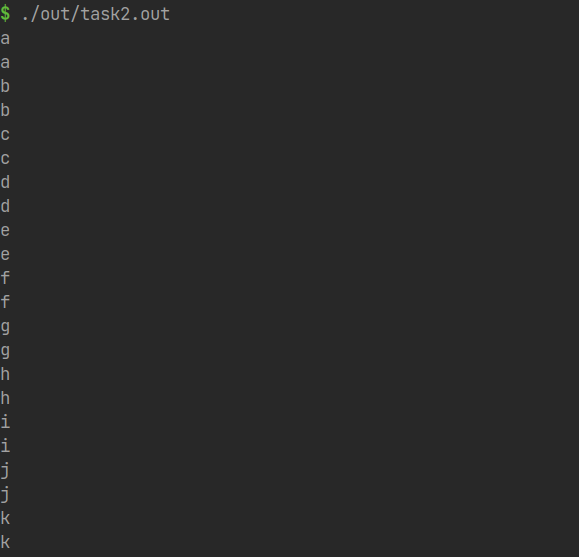
\includegraphics[width=0.7\textwidth]{task2.png}
    \caption{Результат работы второй программы}
\end{figure}

В данной программе процесс получает несколько дескрипторов открытого файла
с использованием системного вызова open. В результате этого чтение происходит
независимо, что проявляется в дублировании выводимых символов.

\subsection{Многопоточная программа}

\begin{lstlisting}[language=c, caption={Вторая программа (многопоточный вариант)}]
#include <stdlib.h>
#include <stdio.h>
#include <fcntl.h>
#include <unistd.h>
#include <pthread.h>

#define MAX_THREADS  12

struct arg
{
    int valid;
    size_t threads;
};

void *thread_func(void *_arg)
{
    int fd = open("alphabet", O_RDONLY);
    char tmp, buf[30];
    ssize_t len;

    if (0 > fd)
    {
        perror("open error\n");

        return NULL;
    }

    for (int read1 = 1; read1;)
        if ((read1 = (1 == read(fd, &tmp, 1))))
        {
            len = sprintf(buf, "thread %zu: %c\n", *(size_t *)_arg, tmp);
            write(1, buf, len);
        }

    close(fd);

    return NULL;
}

int main(int argc, char **argv)
{
    const struct arg arg = parse_args(argc, argv);

    if (EXIT_SUCCESS != arg.valid)
        return EXIT_FAILURE;

    size_t args[MAX_THREADS];
    pthread_t threads[MAX_THREADS];
    int rc = EXIT_SUCCESS;

    for (size_t i = 0; EXIT_SUCCESS == rc && arg.threads > i; i++)
    {
        args[i] = i + 1;

        if (EXIT_SUCCESS
            != pthread_create(threads + i, NULL, thread_func, args + i))
        {
            perror("pthread_create error\n");
            rc = EXIT_FAILURE;
        }
    }

    for (size_t i = 0; arg.threads > i; i++)
        pthread_join(threads[i], NULL);

    return rc;
}
\end{lstlisting}

\begin{figure}[h]
    \centering
    \hspace*{\fill}
    \begin{minipage}{0.45\textwidth}
        \centering
        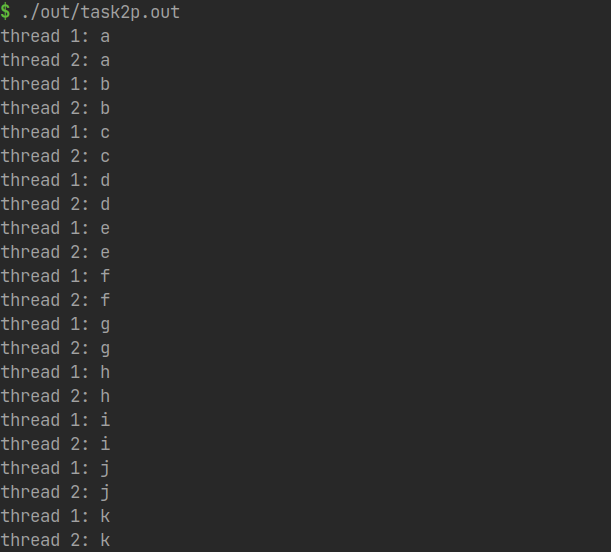
\includegraphics[width=\linewidth]{task2p1.png}
    \end{minipage}
    \hfill
    \begin{minipage}{0.4\textwidth}
        \centering
        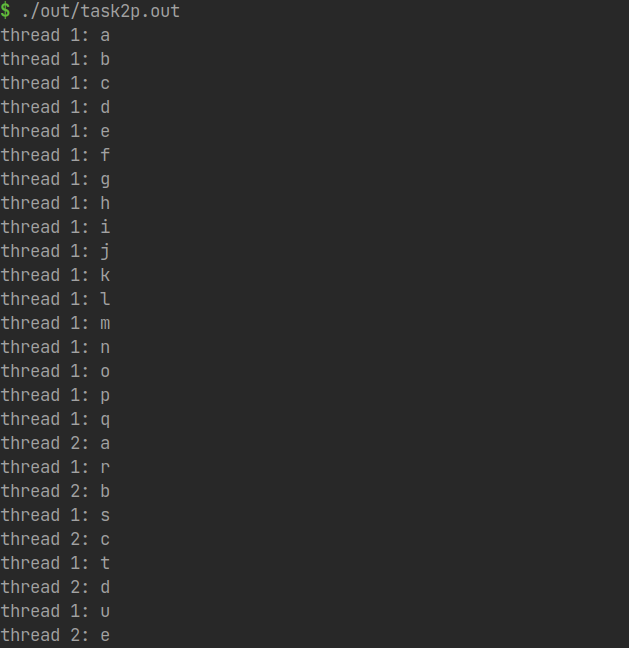
\includegraphics[width=\linewidth]{task2p2.png}
    \end{minipage}
    \hspace*{\fill}
    \caption{Результат работы второй программы.}
\end{figure}

Аналогично однопоточной программе, потоки не мешают друг другу читать из файла,
так как они получают независимые дескрипторы. Внутри одного потока все символы
выводятся подряд в порядке следования, однако из-за асинхронности выполнения
потоков, порядок вывода символов не определен.

\subsection{Связь структур}

\vspace*{\fill}
\begin{figure}[h]
    \centering
    \def\svgwidth{\textwidth}
    \leftsection{Программа 2}

\subsection{Однопоточная программа}

\begin{lstlisting}[language=c, caption={Вторая программа (однопоточный вариант)}]
#include <stdlib.h>
#include <stdio.h>
#include <fcntl.h>
#include <unistd.h>

#define MAX_FDS 10

struct arg
{
    int valid;
    size_t amount;
};

int main(int argc, char **argv)
{
    const struct arg arg = parse_args(argc, argv);

    if (EXIT_SUCCESS != arg.valid)
        return EXIT_FAILURE;

    int fds[MAX_FDS] = {-1};
    char buf[2] = "\0\n";
    int rc = EXIT_SUCCESS;

    for (size_t i = 0; EXIT_SUCCESS == rc && arg.amount > i; i++)
    {
        fds[i] = open("alphabet", O_RDONLY);

        if (0 > fds[i])
        {
            perror("open error");
            rc = EXIT_FAILURE;
        }
    }

    if (EXIT_SUCCESS == rc)
        for (int r = 1; r && !(r = 0);)
            for (size_t i = 0; arg.amount > i; i++)
                if (1 == read(fds[i], buf, 1))
                {
                    write(1, buf, 2);
                    r = 1;
                }

    for (size_t i = 0; arg.amount > i; i++)
        if (fds[i] >= 0)
            close(fds[i]);

    return rc;
}
\end{lstlisting}

\begin{figure}[h]
    \centering
    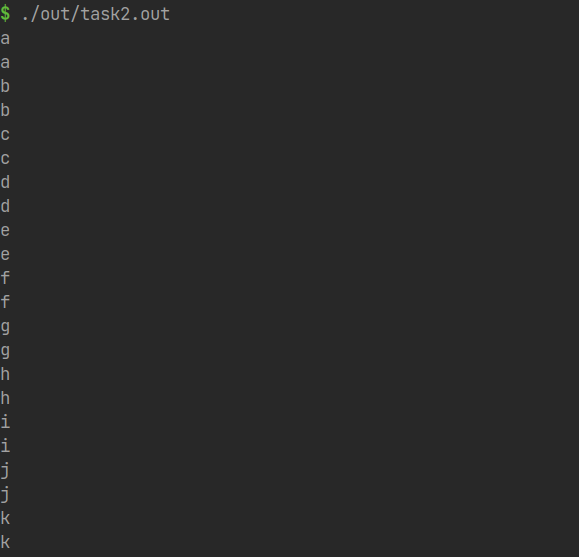
\includegraphics[width=0.7\textwidth]{task2.png}
    \caption{Результат работы второй программы}
\end{figure}

В данной программе процесс получает несколько дескрипторов открытого файла
с использованием системного вызова open. В результате этого чтение происходит
независимо, что проявляется в дублировании выводимых символов.

\subsection{Многопоточная программа}

\begin{lstlisting}[language=c, caption={Вторая программа (многопоточный вариант)}]
#include <stdlib.h>
#include <stdio.h>
#include <fcntl.h>
#include <unistd.h>
#include <pthread.h>

#define MAX_THREADS  12

struct arg
{
    int valid;
    size_t threads;
};

void *thread_func(void *_arg)
{
    int fd = open("alphabet", O_RDONLY);
    char tmp, buf[30];
    ssize_t len;

    if (0 > fd)
    {
        perror("open error\n");

        return NULL;
    }

    for (int read1 = 1; read1;)
        if ((read1 = (1 == read(fd, &tmp, 1))))
        {
            len = sprintf(buf, "thread %zu: %c\n", *(size_t *)_arg, tmp);
            write(1, buf, len);
        }

    close(fd);

    return NULL;
}

int main(int argc, char **argv)
{
    const struct arg arg = parse_args(argc, argv);

    if (EXIT_SUCCESS != arg.valid)
        return EXIT_FAILURE;

    size_t args[MAX_THREADS];
    pthread_t threads[MAX_THREADS];
    int rc = EXIT_SUCCESS;

    for (size_t i = 0; EXIT_SUCCESS == rc && arg.threads > i; i++)
    {
        args[i] = i + 1;

        if (EXIT_SUCCESS
            != pthread_create(threads + i, NULL, thread_func, args + i))
        {
            perror("pthread_create error\n");
            rc = EXIT_FAILURE;
        }
    }

    for (size_t i = 0; arg.threads > i; i++)
        pthread_join(threads[i], NULL);

    return rc;
}
\end{lstlisting}

\begin{figure}[h]
    \centering
    \hspace*{\fill}
    \begin{minipage}{0.45\textwidth}
        \centering
        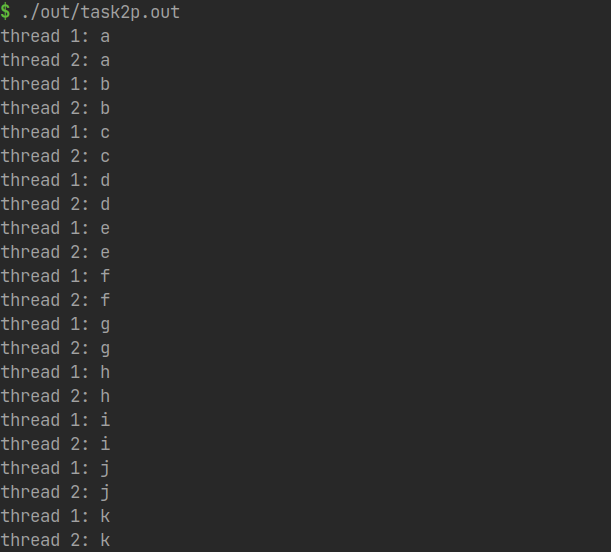
\includegraphics[width=\linewidth]{task2p1.png}
    \end{minipage}
    \hfill
    \begin{minipage}{0.4\textwidth}
        \centering
        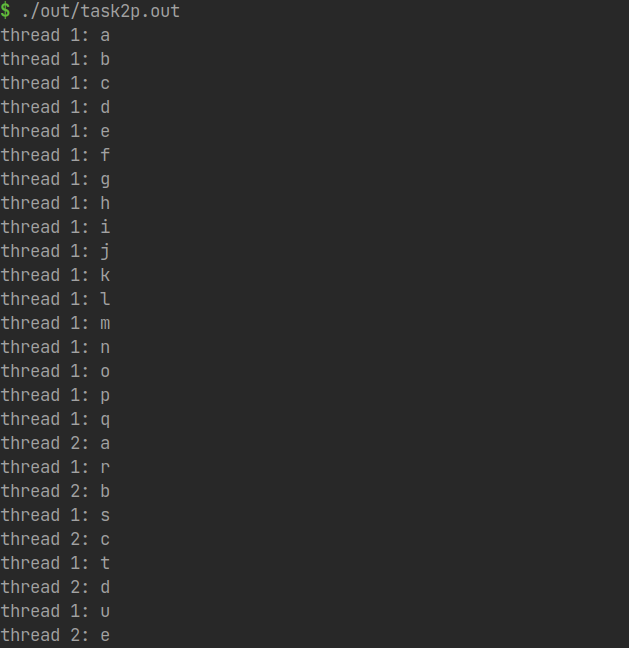
\includegraphics[width=\linewidth]{task2p2.png}
    \end{minipage}
    \hspace*{\fill}
    \caption{Результат работы второй программы.}
\end{figure}

Аналогично однопоточной программе, потоки не мешают друг другу читать из файла,
так как они получают независимые дескрипторы. Внутри одного потока все символы
выводятся подряд в порядке следования, однако из-за асинхронности выполнения
потоков, порядок вывода символов не определен.

\subsection{Связь структур}

\vspace*{\fill}
\begin{figure}[h]
    \centering
    \def\svgwidth{\textwidth}
    \leftsection{Программа 2}

\subsection{Однопоточная программа}

\begin{lstlisting}[language=c, caption={Вторая программа (однопоточный вариант)}]
#include <stdlib.h>
#include <stdio.h>
#include <fcntl.h>
#include <unistd.h>

#define MAX_FDS 10

struct arg
{
    int valid;
    size_t amount;
};

int main(int argc, char **argv)
{
    const struct arg arg = parse_args(argc, argv);

    if (EXIT_SUCCESS != arg.valid)
        return EXIT_FAILURE;

    int fds[MAX_FDS] = {-1};
    char buf[2] = "\0\n";
    int rc = EXIT_SUCCESS;

    for (size_t i = 0; EXIT_SUCCESS == rc && arg.amount > i; i++)
    {
        fds[i] = open("alphabet", O_RDONLY);

        if (0 > fds[i])
        {
            perror("open error");
            rc = EXIT_FAILURE;
        }
    }

    if (EXIT_SUCCESS == rc)
        for (int r = 1; r && !(r = 0);)
            for (size_t i = 0; arg.amount > i; i++)
                if (1 == read(fds[i], buf, 1))
                {
                    write(1, buf, 2);
                    r = 1;
                }

    for (size_t i = 0; arg.amount > i; i++)
        if (fds[i] >= 0)
            close(fds[i]);

    return rc;
}
\end{lstlisting}

\begin{figure}[h]
    \centering
    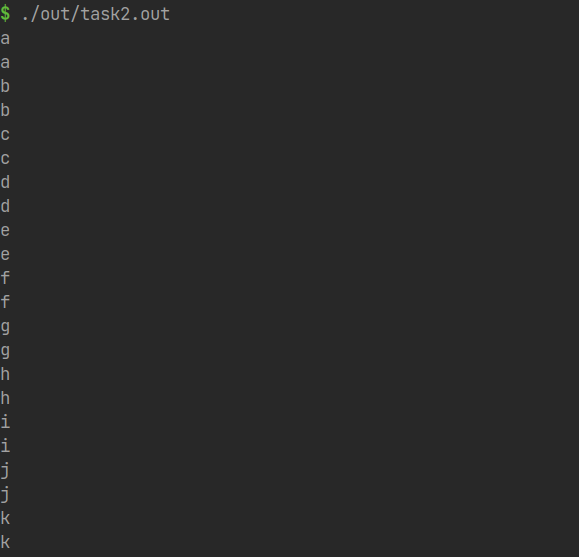
\includegraphics[width=0.7\textwidth]{task2.png}
    \caption{Результат работы второй программы}
\end{figure}

В данной программе процесс получает несколько дескрипторов открытого файла
с использованием системного вызова open. В результате этого чтение происходит
независимо, что проявляется в дублировании выводимых символов.

\subsection{Многопоточная программа}

\begin{lstlisting}[language=c, caption={Вторая программа (многопоточный вариант)}]
#include <stdlib.h>
#include <stdio.h>
#include <fcntl.h>
#include <unistd.h>
#include <pthread.h>

#define MAX_THREADS  12

struct arg
{
    int valid;
    size_t threads;
};

void *thread_func(void *_arg)
{
    int fd = open("alphabet", O_RDONLY);
    char tmp, buf[30];
    ssize_t len;

    if (0 > fd)
    {
        perror("open error\n");

        return NULL;
    }

    for (int read1 = 1; read1;)
        if ((read1 = (1 == read(fd, &tmp, 1))))
        {
            len = sprintf(buf, "thread %zu: %c\n", *(size_t *)_arg, tmp);
            write(1, buf, len);
        }

    close(fd);

    return NULL;
}

int main(int argc, char **argv)
{
    const struct arg arg = parse_args(argc, argv);

    if (EXIT_SUCCESS != arg.valid)
        return EXIT_FAILURE;

    size_t args[MAX_THREADS];
    pthread_t threads[MAX_THREADS];
    int rc = EXIT_SUCCESS;

    for (size_t i = 0; EXIT_SUCCESS == rc && arg.threads > i; i++)
    {
        args[i] = i + 1;

        if (EXIT_SUCCESS
            != pthread_create(threads + i, NULL, thread_func, args + i))
        {
            perror("pthread_create error\n");
            rc = EXIT_FAILURE;
        }
    }

    for (size_t i = 0; arg.threads > i; i++)
        pthread_join(threads[i], NULL);

    return rc;
}
\end{lstlisting}

\begin{figure}[h]
    \centering
    \hspace*{\fill}
    \begin{minipage}{0.45\textwidth}
        \centering
        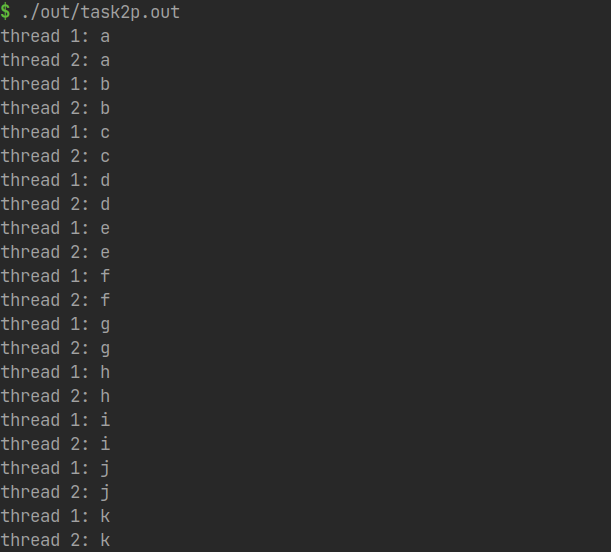
\includegraphics[width=\linewidth]{task2p1.png}
    \end{minipage}
    \hfill
    \begin{minipage}{0.4\textwidth}
        \centering
        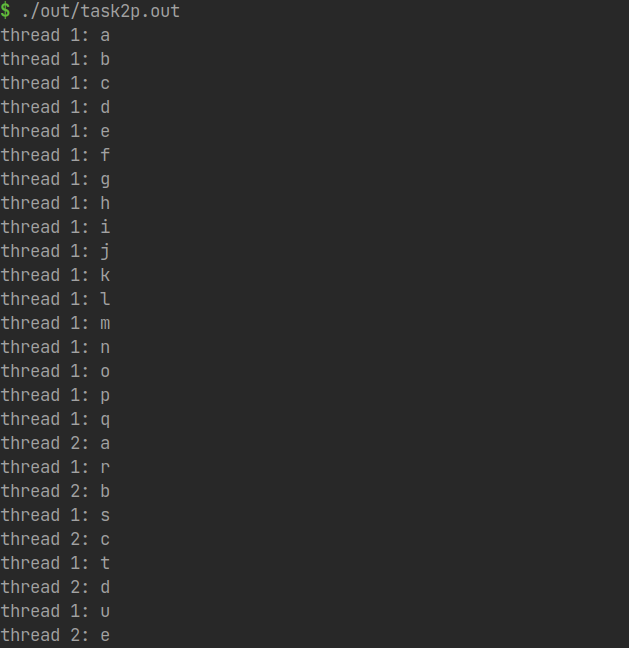
\includegraphics[width=\linewidth]{task2p2.png}
    \end{minipage}
    \hspace*{\fill}
    \caption{Результат работы второй программы.}
\end{figure}

Аналогично однопоточной программе, потоки не мешают друг другу читать из файла,
так как они получают независимые дескрипторы. Внутри одного потока все символы
выводятся подряд в порядке следования, однако из-за асинхронности выполнения
потоков, порядок вывода символов не определен.

\subsection{Связь структур}

\vspace*{\fill}
\begin{figure}[h]
    \centering
    \def\svgwidth{\textwidth}
    \leftsection{Программа 2}

\subsection{Однопоточная программа}

\begin{lstlisting}[language=c, caption={Вторая программа (однопоточный вариант)}]
#include <stdlib.h>
#include <stdio.h>
#include <fcntl.h>
#include <unistd.h>

#define MAX_FDS 10

struct arg
{
    int valid;
    size_t amount;
};

int main(int argc, char **argv)
{
    const struct arg arg = parse_args(argc, argv);

    if (EXIT_SUCCESS != arg.valid)
        return EXIT_FAILURE;

    int fds[MAX_FDS] = {-1};
    char buf[2] = "\0\n";
    int rc = EXIT_SUCCESS;

    for (size_t i = 0; EXIT_SUCCESS == rc && arg.amount > i; i++)
    {
        fds[i] = open("alphabet", O_RDONLY);

        if (0 > fds[i])
        {
            perror("open error");
            rc = EXIT_FAILURE;
        }
    }

    if (EXIT_SUCCESS == rc)
        for (int r = 1; r && !(r = 0);)
            for (size_t i = 0; arg.amount > i; i++)
                if (1 == read(fds[i], buf, 1))
                {
                    write(1, buf, 2);
                    r = 1;
                }

    for (size_t i = 0; arg.amount > i; i++)
        if (fds[i] >= 0)
            close(fds[i]);

    return rc;
}
\end{lstlisting}

\begin{figure}[h]
    \centering
    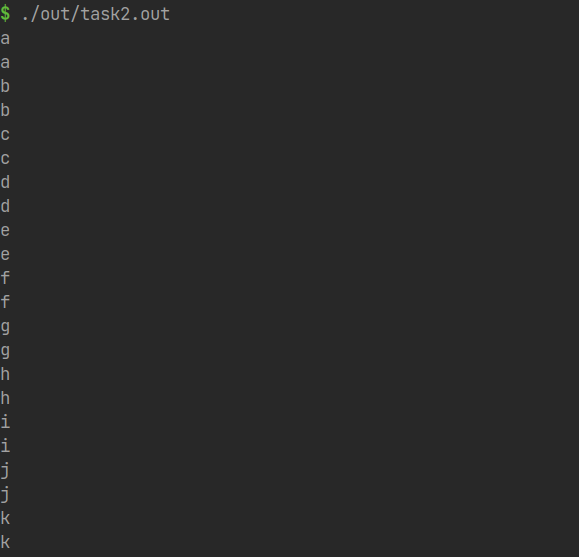
\includegraphics[width=0.7\textwidth]{task2.png}
    \caption{Результат работы второй программы}
\end{figure}

В данной программе процесс получает несколько дескрипторов открытого файла
с использованием системного вызова open. В результате этого чтение происходит
независимо, что проявляется в дублировании выводимых символов.

\subsection{Многопоточная программа}

\begin{lstlisting}[language=c, caption={Вторая программа (многопоточный вариант)}]
#include <stdlib.h>
#include <stdio.h>
#include <fcntl.h>
#include <unistd.h>
#include <pthread.h>

#define MAX_THREADS  12

struct arg
{
    int valid;
    size_t threads;
};

void *thread_func(void *_arg)
{
    int fd = open("alphabet", O_RDONLY);
    char tmp, buf[30];
    ssize_t len;

    if (0 > fd)
    {
        perror("open error\n");

        return NULL;
    }

    for (int read1 = 1; read1;)
        if ((read1 = (1 == read(fd, &tmp, 1))))
        {
            len = sprintf(buf, "thread %zu: %c\n", *(size_t *)_arg, tmp);
            write(1, buf, len);
        }

    close(fd);

    return NULL;
}

int main(int argc, char **argv)
{
    const struct arg arg = parse_args(argc, argv);

    if (EXIT_SUCCESS != arg.valid)
        return EXIT_FAILURE;

    size_t args[MAX_THREADS];
    pthread_t threads[MAX_THREADS];
    int rc = EXIT_SUCCESS;

    for (size_t i = 0; EXIT_SUCCESS == rc && arg.threads > i; i++)
    {
        args[i] = i + 1;

        if (EXIT_SUCCESS
            != pthread_create(threads + i, NULL, thread_func, args + i))
        {
            perror("pthread_create error\n");
            rc = EXIT_FAILURE;
        }
    }

    for (size_t i = 0; arg.threads > i; i++)
        pthread_join(threads[i], NULL);

    return rc;
}
\end{lstlisting}

\begin{figure}[h]
    \centering
    \hspace*{\fill}
    \begin{minipage}{0.45\textwidth}
        \centering
        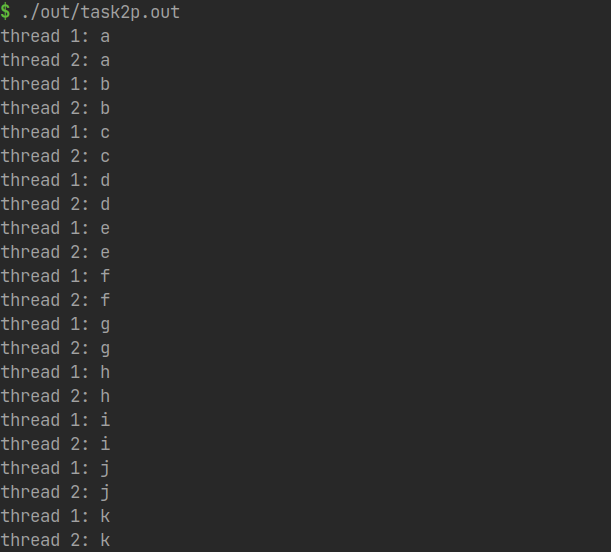
\includegraphics[width=\linewidth]{task2p1.png}
    \end{minipage}
    \hfill
    \begin{minipage}{0.4\textwidth}
        \centering
        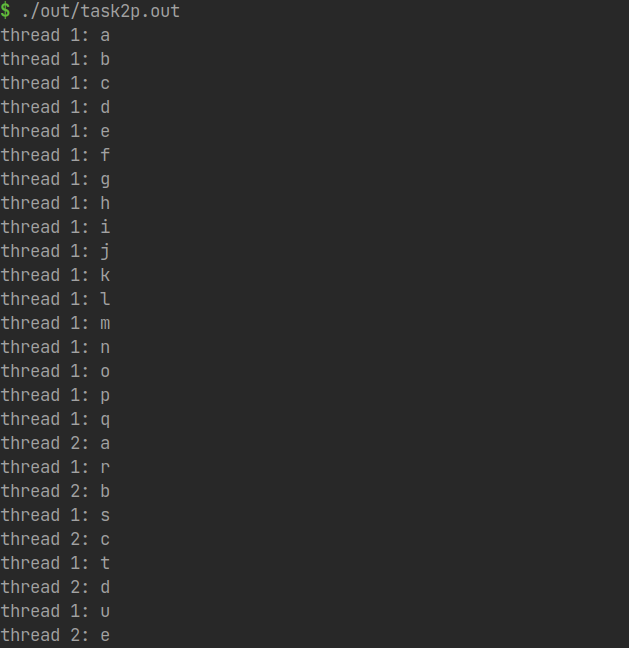
\includegraphics[width=\linewidth]{task2p2.png}
    \end{minipage}
    \hspace*{\fill}
    \caption{Результат работы второй программы.}
\end{figure}

Аналогично однопоточной программе, потоки не мешают друг другу читать из файла,
так как они получают независимые дескрипторы. Внутри одного потока все символы
выводятся подряд в порядке следования, однако из-за асинхронности выполнения
потоков, порядок вывода символов не определен.

\subsection{Связь структур}

\vspace*{\fill}
\begin{figure}[h]
    \centering
    \def\svgwidth{\textwidth}
    \input{task2.pdf_tex}
\end{figure}
\vfill


\end{figure}
\vfill


\end{figure}
\vfill


\end{figure}
\vfill

